\section{Uma avaliação do OpenFlow}

\begin{frame}{Proposta}

    \begin{itemize}
        \item Avaliar o protocolo OpenFlow através de um sistema de
            balanceamento de carga.
        \item Através dos recursos fornecidos pelo protocolo é possível 
            maximizar a justiça no balanceamento de carga em um serviço HTTP.
    \end{itemize}

    \begin{figure}[!htb]
        \centering
        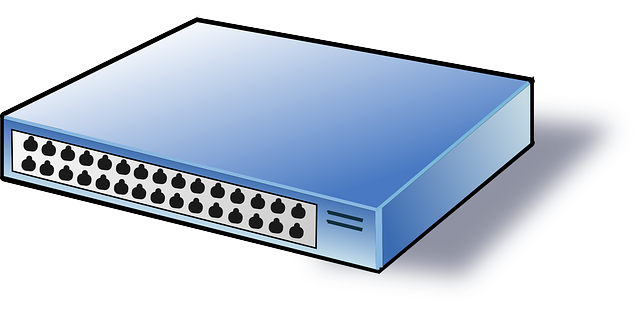
\includegraphics[scale=.3]{images/cartoon-switch}
    \end{figure}
\end{frame}


\begin{frame}{Introdução}
    \begin{itemize}
        \setlength{\itemsep}{.5cm}
        \item Sistemas de balanceamento de carga são baseados em políticas 
            de balanceamento.
        \item Os serviços modernos devem ser escaláveis para atender a 
            milhões ou milhares de clientes.
        \item Os serviços devem ser distribuídos em vários servidores. 
        \item O OpenFlow permite políticas que podem se adaptar à aplicação 
            ou serviço.
    \end{itemize} 
\end{frame}
